\section{The Fast Multipole Method}\label{chpt:2:sec:0}

In this section we introduce the Fast Multipole Method (FMM), a foundational fast algorithm, the implementation of which is central to our software infrastructure. We begin by describing the FMM, first introduced by Greengard and Rokhlin in the 1980s, in the context of the solution of the $N$-body potential calculation problem of electrostatics, or gravitation, which gives rise to much of the terminology in this field \cite{greengard1987fast}. We proceed to describe more modern algorithmic approaches, which retain many of the core algorithmic features of the original FMM while being more amenable to software implementation on modern computer hardware \cite{Ying:2004:JCP,fong2009black}. We note that the FMM in its most basic form corresponds to a matrix-vector product, and we therefore conclude by briefly contrasting the FMM with similar methods for computing this quantity, as well as noting methods for computing the approximate inverse of FMM matrices, which correspond to a form of direct solver, termed `fast direct solvers'.

Consider the following $N$-body problem which appears in the calculation of electrostatic, or gravitational potentials from a set of point charges, or masses,

\begin{flalign}\label{eq:chpt:2:sec:0:fmm_problem}
    \phi_j = \sum_{i=1}^N K(x_i, x_j) q_i
\end{flalign}

Here, $q_i$ is a point charge/mass, corresponding to $N$ particles at positions $x_i$ and the `kernel' is defined as,


\begin{flalign}\label{eq:chpt:2:sec:0:laplace_kernel}
    K(x,y) =
    \left\{
        \begin{array}{ll}
            \log\|x-y\| & \text{in } \mathbb{R}^2 \\
            \frac{1}{4\pi\|x-y\|} & \text{in } \mathbb{R}^3
        \end{array}
    \right.
\end{flalign}

Writing the component form (\ref{eq:chpt:2:sec:0:laplace_kernel}) as its corresponding linear system,

\begin{flalign}\label{eq:chpt:2:sec:0:fmm_linear_system}
   \mathbf{\phi} = K \mathbf{q}
\end{flalign}

We note that the matrix $K$ is \textit{dense}, with non-zero off diagonal elements, and that this implies a global data dependency between all point charges/masses. This global data dependency had previously inhibited numerical methods for $N$-body problems as a naive application of this matrix requires $O(N^2)$ flops, and an finding an inverse using a linear algebra technique such as LU decomposition or Gaussian Elimination requires $O(N^3)$ flops. The key insight behind the FMM, and subsequent fast algorithms, was that the interactions between physically distant groups of points could be compressed with a bounded accuracy if the kernel function exhibits amenable properties, specifically if it rapidly decays as the distance between two point sets increases. We demonstrate this in figure \ref{fig:chpt:2:sec:0:rank_decay}.

\begin{figure}[h]
    \centering
    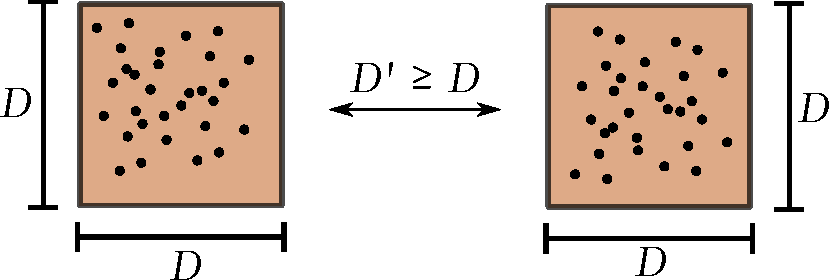
\includegraphics[width=0.7\linewidth]{images/ch_2/low_rank.pdf}
    \caption{Given two boxes in $\mathbb{R}^d$ ($d=2$ or 3), $\mathcal{B}_1$ and $\mathcal{B}_2$, which each enclose a corresponding set of points. The off-diagonal blocks in the matrix $K_{\mathcal{B}_1\mathcal{B}_2}$ and $K_{\mathcal{B}_2\mathcal{B}_1}$ are considered low rank and amenable to compression for the FMM when the distance separating them is at least equal to their diameter.}
    \label{fig:chpt:2:sec:0:rank_decay}
\end{figure}

From figure \ref{fig:chpt:2:sec:0:rank_decay} we see that the FMM relies on a discretisation that allows us to systematically compress far-interactions. To see how we obtain this, we start by placing our problem in a square/cube domain containing all $N$ points, denoting this with $\Omega$. Returning to (\ref{eq:chpt:2:sec:0:fmm_linear_system}), we must calculate the potential vector $\phi \in \mathbb{R}^N$, from a charge/mass vector $\mathbf{q} \in \mathbb{R}^N$ by applying $K \in \mathbb{R}^{N \times N} $. We begin with the situation in figure \ref{fig:chpt:2:sec:0:rank_decay}, where we have two sets of particles contained in boxes separated by some distance that makes their interaction amenable to compression, the FMM literature often describes such boxes as being `well separated'. Labelling the boxes as $\Omega_s$ and $\Omega_t$, containing `source' particles $\{y_j\}_{j=1}^M$, with associated charges/masses $q_j$, and `target' particles $\{x_i\}_{i=1}^N$ respectively, we seek to evaluate the potential introduced by the source particles at the target particles. As the interaction assumed to be amenable to compression we are able to write an approximation to (\ref{eq:chpt:2:sec:0:fmm_problem}) using a low-rank approximation for the kernel in terms of tensor products as,

\begin{flalign}
    K(x, y) \approx \sum_{p=0}^{P-1} B_p(x) C_p(y), \> \> \text{ when } x \in \Omega_t, \> y \in \Omega_s
\end{flalign}

Where $P$ is called the `expansion order', or `interaction rank'. This is equivalent to approximating the kernel with an SVD using its leading singular values. We introduce index sets $I_s$ and $I_t$ which label the points inside $\Omega_s$ and $\Omega_t$ respectively, and find a generic approximation for the charges/masses,

\begin{flalign}
    \hat{q}_p = \sum_{j \in I_s}C_p(x_j)q_j, \> p=0, 1, 2...P-1
\end{flalign}

Using this we can evaluate an approximation to the potential due to these particles in the far-field as,

\begin{flalign}
    \phi_i \approx \sum_{p=1}^{P-1}B_p(x_i)\hat{q}_p
\end{flalign}

In doing so we accelerate (\ref{eq:chpt:2:sec:0:fmm_problem}) from $O(MN)$ to $O(P(M + N))$. As long as we choose $P \ll M$ and $P \ll N$, we recover an accelerated matrix vector product for calculating the potential interactions between the set of sources and targets from two well separated boxes. The rapid decay behaviour of the kernel ensures that we can recover the potential in $\Omega_t$ with high-accuracy even if $P$ is small. We note that although we represent the sources/targets as corresponding to different particle sets in this derivation they may be equivalent.

We deliberately haven't stated how we calculate $B_p$ or $C_p$. In Greengard and Rokhlin's original FMM these took the form of analytical multipole and local expansions of the kernel function \cite{greengard1987fast}. To demonstrate this we derive an expansion in the $\mathbb{R}^2$ case, taking $c_s$ and $c_t$ as the centres of $\Omega_s$ and $\Omega_t$ respectively,

\begin{flalign}
    \label{eq:ch_2:analytical_multipole_expansion}
    K(x,y) = \log(x-y) &= \log((x-c_s) - (y-c_s)) \\ \nonumber &= \log(x-c_s) + \log(1-\frac{y-c_s}{x-c_s}) \\
    \nonumber &= \log(x-c_s) - \sum_{p=1}^\infty \frac{1}{p}\frac{(y-c_s)^p}{(x-c_s)^p}
\end{flalign}

where the series converges for $|y-c_s| < |c-c_s|$. We note (\ref{eq:ch_2:analytical_multipole_expansion}) is exactly of the form required with $C_p(y) = -\frac{1}{p}(y-c_s)^p$ and $B_p(x) = (x-c_s)^{-p}$. We define a `multipole expansion' of the charges in $\Omega_s$ as a vector $\mathsf{\hat{q}^s} = \{ \hat{q}_p^s \}_{p=0}^{P-1}$,

\begin{flalign}
    \begin{dcases}
        \hat{q}_0^s = \sum_{j \in I_s} q_j \\
        \hat{q}_p^s = \sum_{j \in I_s} - \frac{1}{p}(x_j - c_s)^p q_j, \> \> p = 1,2,3...,P-1
    \end{dcases}
\end{flalign}

The multipole expansion is a representation of the charges in $\Omega_s$ and can be truncated to any required precision. We can use the multipole expansion in place of a direct calculation with the particles in $\Omega_s$. As the potential in $\Omega_t$ can be written as,

\begin{flalign}\label{eq:ch_2:multipole_expansions}
    \phi(x) = \sum_{j \in I_s} K(x, y)q_j = \log(x-c_s)\hat{q}_0^s + \sum_{p=1}^\infty \frac{1}{(x-c_s)^p}\hat{q}_p^s
\end{flalign}

Greengard and Rokhlin also define a local expansion centered on $\Omega_t$, that represents the potential due to the sources in $\Omega_s$.

\begin{flalign}
    \phi(x) = \sum_{l=1}^\infty (x-c_t)^l \hat{\phi}^t_l
\end{flalign}

with a simple computation to derive the local expansion coefficients $\{\hat{\phi}^t_p\}_{p=0}^\infty$ from $\{ \hat{q}_p^s \}_{p=0}^{P-1}$ (see app. \ref{app:locals}).

For our purposes it's useful to write the multipole expansion in linear algebraic terms as a linear map between vectors,

\begin{flalign}
    \mathsf{\hat{q}}^s = \mathsf{T}^{P2M}_s\mathsf{q}(I_s)
\end{flalign}

where $\mathsf{T}_s^{P2M}$ is a $P \times N_s$ matrix, analogously for the local expansion coefficients we can write,

\begin{flalign}
    \mathsf{\hat{\phi}}^t = \mathsf{T}_{t,s}^{M2L}\mathsf{\hat{q}}^s
\end{flalign}

where $\mathsf{T}_{t,s}^{M2L}$ is a $P \times P$ matrix, and the calculation of the final potentials as,

\begin{flalign}
    \mathsf{\phi}^t = \mathsf{T}_t^{L2P}\mathsf{\hat{\phi}}^t
\end{flalign}

where $\mathsf{T}_t^{L2P}$ is a $N_t \times P$ matrix. Here we denote each \textit{translation} operator, $\mathsf{T}^{X2Y}$, with a label read as `$X$ to $Y$' where $L$ stands for local, $M$ for multipole and $P$ for particle. Written in this form, we observe that one could use a different method to approximate the translation operators than explicit kernel expansions to recover our approach's algorithmic complexity, and this is indeed the main difference between different implementations of the FMM.

We have described how to obtain linear complexity when considering two isolated boxes, however in order to recover this for interactions between \textit{all particles}  we rely on a hierarchical partitioning of $\Omega$ using a data structure from computer science called a \textit{quadtree} in $\mathbb{R}^2$ or an \textit{octree} in $\mathbb{R}^3$. The defining feature of these data structures is a recursive partition of a bounding box drawn over the region of interest (see fig. \ref{fig:chpt:2:sec:0:octree_example}). This ‘root node/box’ is subdivided into four equal parts in $\mathbb{R}^2$ and eight equal parts in $\mathbb{R}^3$. These ‘child nodes/boxes’ turn are in turn recursively subdivided until a user defined threshold is reached based on the maximum number of points per leaf box. These trees can be `adaptive' by allowing for non-uniform leaf box sizes, and `balanced' to enforce a maximum size constraint between adjacent leaf boxes \cite{sundar2008bottom}.

\begin{figure}
    \centering
    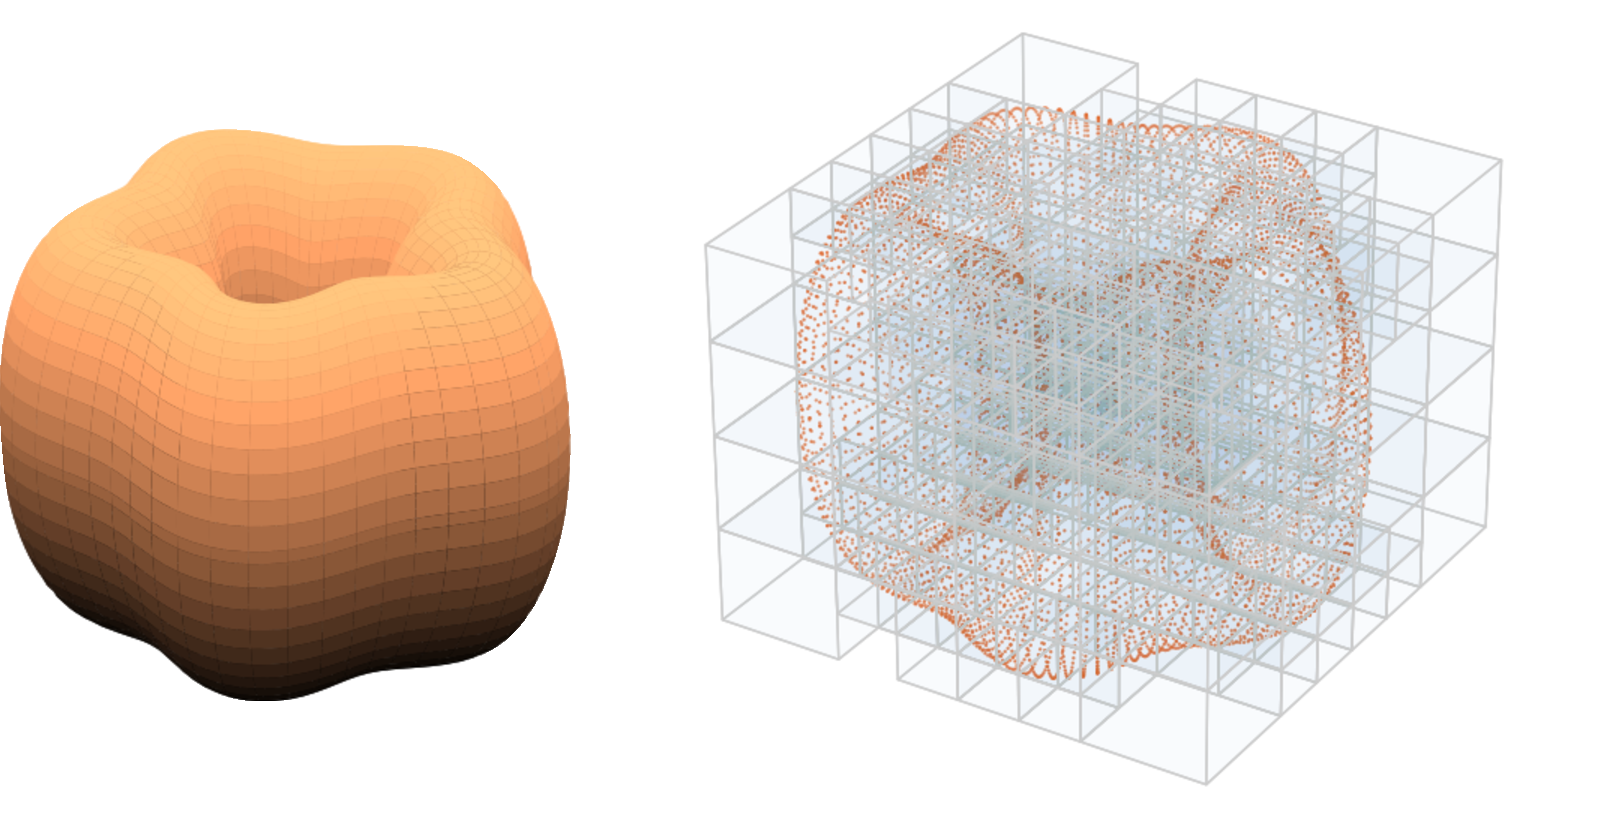
\includegraphics[width=0.7\textwidth]{ch_2/octree_example.pdf}
    \caption{An adaptive octree for random point data placed on the surface of a `wiggly torus' test geometry. The user defines the level of recursion via a threshold for the maximum number of particles in a given node.}
    \label{fig:chpt:2:sec:0:octree_example}
\end{figure}

In addition to the $\mathsf{T}^{P2M}$, $\mathsf{T}^{M2L}$ and $\mathsf{T}^{L2P}$ the FMM also require operators that can translate the expansion centre of a multipole or local expansion, $\mathsf{T}^{L2L}$, $\mathsf{T}^{M2M}$, an operator that can add the contribution of a set of points to a given local expansion $\mathsf{T}^{P2L}$, and apply a multipole approximation to a set of points, $\mathsf{T}^{M2P}$, finally we need define a $P2P$ operator, which is short hand for direct kernel evaluations. Algorithm (\ref{alg:fmm}) in Appendix \ref{app:adaptive_fmm} provides a sketch of the full FMM algorithm which combines these operators.

In summary the algorithm consists of two basic steps. During the first step, the upward pass, the tree is traversed in post-order \footnote{The children of a box are visited before the box itself.}. At the leaves, multipole expansions are built using $\mathsf{T}^{P2M}$. At each non-leaf box, the multipole expansions are shifted to the box's centre from its children using $\mathsf{T}^{M2M}$ and summed. In the second step, the downward pass, the tree is traversed in pre-order\footnote{The children of a box are visited after the box itself.}. The local expansions are computed by first translating the multipole expansions of boxes which are the children of the parents of a box, but are not adjacent to it, using $\mathsf{T}^{M2L}$ and are summed, a second contribution is found from a box's parent using $\mathsf{T}^{L2L}$ to shift the expansion centre from a box's parent to its own centre. It is common to refer to boxes for which $T^{M2L}$ is applied to for a given box $B$ as its \textit{interaction list}. The sum of these two parts encodes all the contribution from sources particles in boxes with are not adjacent to itself. For non-uniform trees there also may be a contribution from boxes in near field of $B$, i.e. neighbour children/descendants, calculated using $T^{P2L}$. This is computed at the leaf level only. Having assembled the far-field contribution at $B$ in its local expansion we evaluate it at the particles it contains using $\mathsf{T}^{L2P}$, combining it with its near interactions from particles in adjacent boxes using $P2P$, as well as boxes which are non-adjacent but for which the multipole expansion still applies using $\mathsf{T}^{M2P}$ in a box's near-field, i.e. the children and descendants of adjacent boxes at the same level.

The complexity bound of the FMM algorithm is due to the hierarchical nature of the data structure used in its computation. In the upward pass, each box only considers either itself. This leads to a complexity of $O(N)$, as the number of leaf boxes is bounded by the number of particles. In the downward pass, the number of boxes each box considers when computing translations is bounded by the number of non-adjacent children of its parent box for the $T^{M2L}$ step, i.e. the size of its interaction list. As this is a constant (27 in $\mathbb{R}^2$ and 189 in $\mathbb{R}^3$), this step is again $O(N)$ in complexity, resulting in a total complexity of $O(N)$ for this step. In the $T^{L2L}$ and $T^{L2P}$ operators each box considers only itself. For the leaf level computations, the $P2P$ ,$T^{P2L}$ and $T^{M2P}$ steps are bounded to be contained in boxes in $B$'s near field \footnote{In the worst case, for highly non-uniform point distributions, these steps can be subsumed into the $P2P$ step, allowing us to maintain the bound.}. This leads to an overall algorithmic complexity of $O(N)$. We note that this complexity bound is entirely dependent on the properties of the kernel. Highly oscillatory kernels are not as rank-deficient, however corresponding algorithms inspired by the FMM have been developed for them, however here the complexity increases to $O(N \log (N) )$ \cite{messner2012fast}. The conversion of an $O(N^2)$ problem to one that can be solved in $O(N)$ was a groundbreaking discovery, and lead to the admissibility of a large number of scientific problems to computer simulation. As a result the FMM has been described as `one of the top ten algorithmic discoveries of the twentieth century', taking its place alongside revolutionary algorithms such as Quicksort and the Fast Fourier Transform (FFT) \cite{cipra2000best}.